\subsection{Software design descriptions and UML}

In the following pages we present some diagrams that are fundamental to creating appropriate documentation. The following diagrams show how to create some UML diagrams.

\subsubsection{Component Diagram (C\&C structure)}

A \definition{Component Diagram} breaks down the actual \textbf{system} under development into \textbf{various high levels of functionality}. Each component is responsible for one clear aim within the entire system and only interacts with other essential elements on a need-to-know basis.

\begin{figure}[!htp]
    \centering
    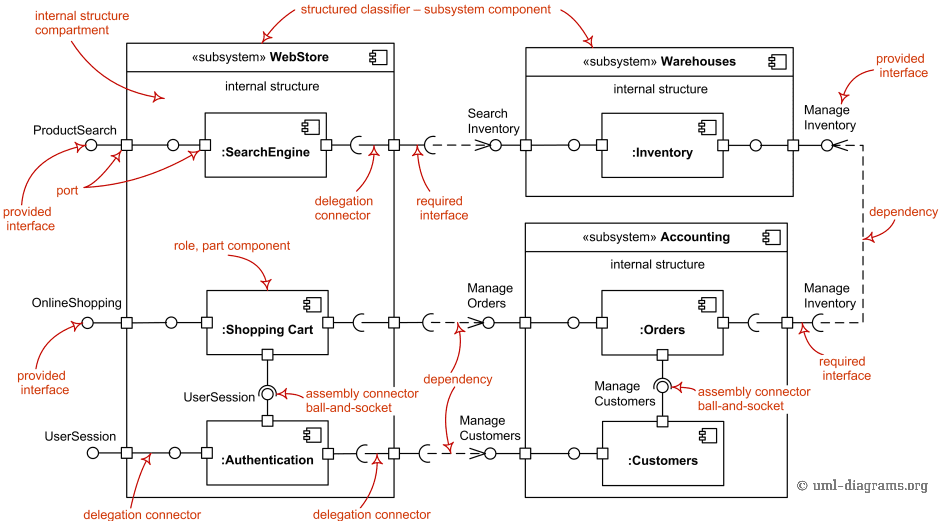
\includegraphics[width=\textwidth]{img/component-diagram.png}
    \caption{Component Diagram.}
\end{figure}

\noindent
To view the component diagram in high resolution, scan (or click) the QR code below.
\begin{center}
    \qrcode{https://github.com/PoliMI-HPC-E-notes-projects-AndreVale69/HPC-E-PoliMI-university-notes/tree/main/software-engineering-for-hpc/notes/img/component-diagram.png}
\end{center}
A complete guide can be found on the following page: \href{https://www.visual-paradigm.com/guide/uml-unified-modeling-language/what-is-component-diagram/}{What is Component Diagram?
}

\newpage

\subsubsection{Sequence Diagram (C\&C structure)}

\definition{Sequence Diagram} show \textbf{elements as they interact over time} and they are organized according to object (horizontally) and time (vertically).

\begin{figure}[!htp]
    \centering
    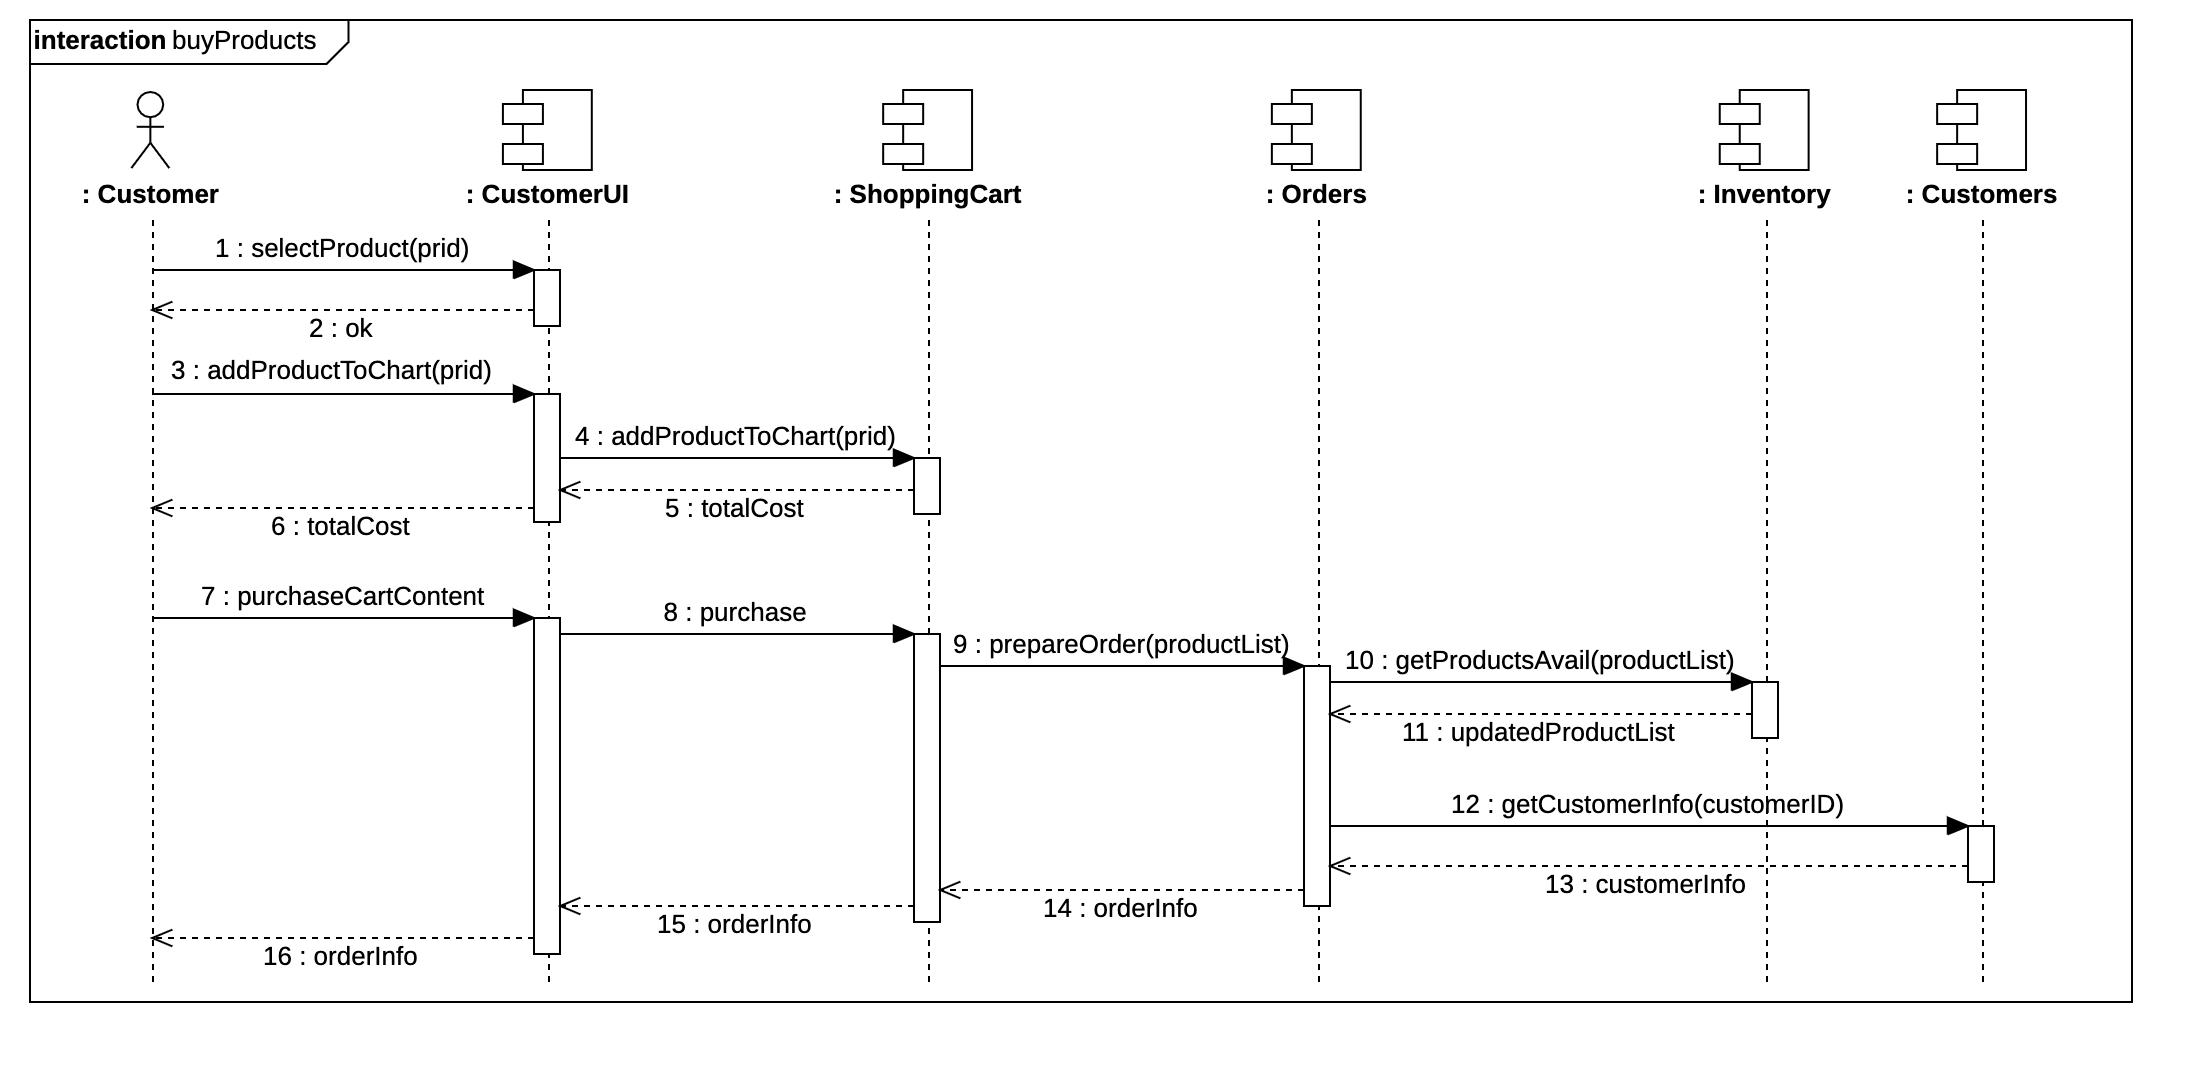
\includegraphics[width=\textwidth]{img/sequence-diagram.png}
    \caption{Sequence Diagram.}
\end{figure}

\noindent
To view the sequence diagram in high resolution, scan (or click) the QR code below.
\begin{center}
    \qrcode{https://github.com/PoliMI-HPC-E-notes-projects-AndreVale69/HPC-E-PoliMI-university-notes/tree/main/software-engineering-for-hpc/notes/img/sequence-diagram.png}
\end{center}
A complete guide can be found on the following page: \href{https://www.visual-paradigm.com/guide/uml-unified-modeling-language/what-is-sequence-diagram/}{What is Sequence Diagram?
}

\newpage

\subsubsection{Class Diagram (module structure)}

A \definition{Class Diagram} is \textbf{a type of static structure diagram} that describes the structure of a system by showing the system's classes, their attributes, operations (or methods), and the relationships among objects.

\begin{figure}[!htp]
    \centering
    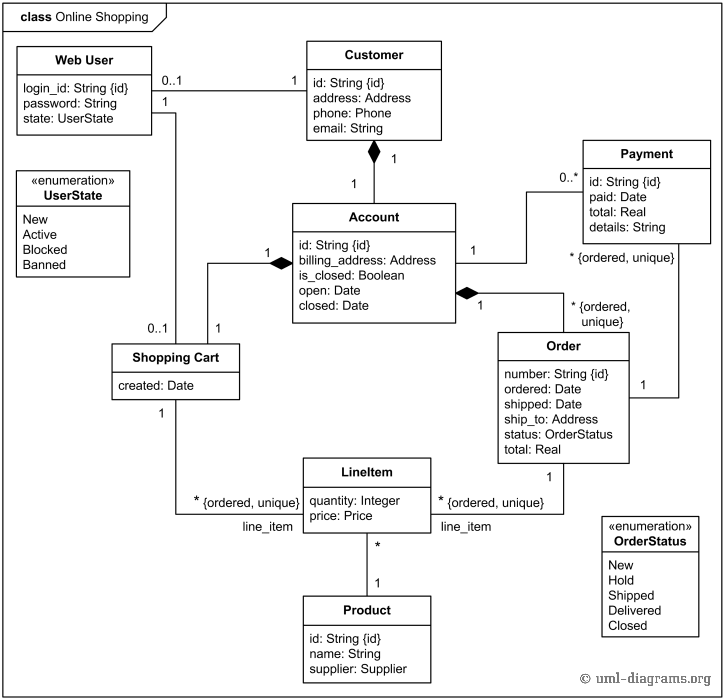
\includegraphics[width=\textwidth]{img/class-diagram.png}
    \caption{Class Diagram.}
\end{figure}

\noindent
To view the sequence diagram in high resolution, scan (or click) the QR code below.
\begin{center}
    \qrcode{https://github.com/PoliMI-HPC-E-notes-projects-AndreVale69/HPC-E-PoliMI-university-notes/tree/main/software-engineering-for-hpc/notes/img/class-diagram.png}
\end{center}
A complete guide can be found on the following page: \href{https://www.visual-paradigm.com/guide/uml-unified-modeling-language/what-is-class-diagram/}{What is Class Diagram?
}

\newpage

\subsubsection{Package Diagram (module structure)}

A \definition{Package Diagram}, a kind of structural diagram, shows the \textbf{arrangement and organization of model elements in middle to large scale project}. Package diagram can show both structure and dependencies between sub-systems or modules, showing different views of a system, for example, as multi-layered (aka multi-tiered) application - multi-layered application model.

\begin{figure}[!htp]
    \centering
    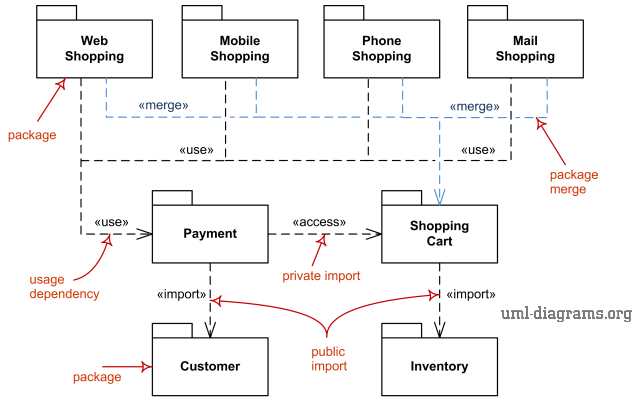
\includegraphics[width=\textwidth]{img/package-diagram.png}
    \caption{Package Diagram.}
\end{figure}

\noindent
To view the sequence diagram in high resolution, scan (or click) the QR code below.
\begin{center}
    \qrcode{https://github.com/PoliMI-HPC-E-notes-projects-AndreVale69/HPC-E-PoliMI-university-notes/tree/main/software-engineering-for-hpc/notes/img/package-diagram.png}
\end{center}
A complete guide can be found on the following page: \href{https://www.visual-paradigm.com/guide/uml-unified-modeling-language/what-is-package-diagram/}{What is Package Diagram?
}

\newpage

\subsubsection{Deployment Diagram (allocation structure)}

A \definition{Deployment Diagram} is a diagram that shows the \textbf{configuration of run time processing nodes and the components that live on them}. Deployment diagrams is a kind of structure diagram used in modeling the physical aspects of an object-oriented system. They are often be used to model the static deployment view of a system (topology of the hardware).

\begin{figure}[!htp]
    \centering
    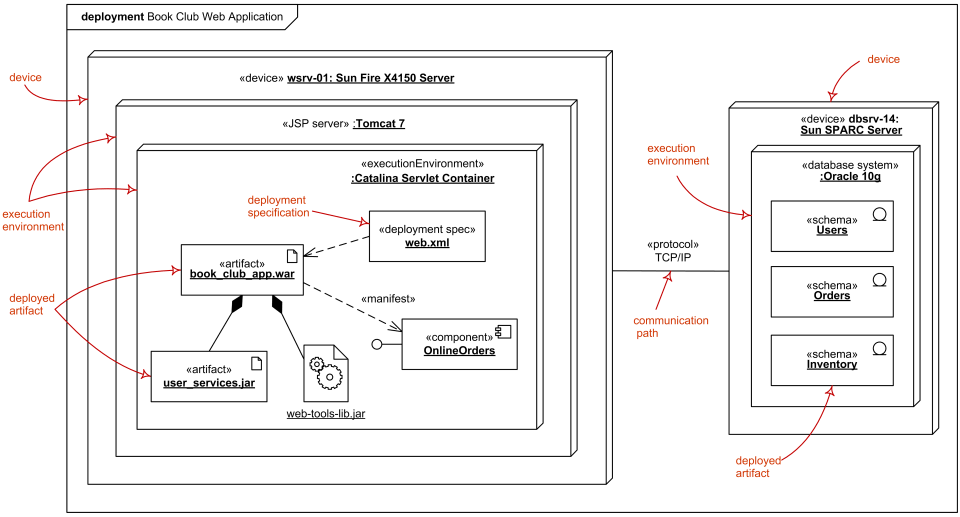
\includegraphics[width=\textwidth]{img/deployment-diagram.png}
    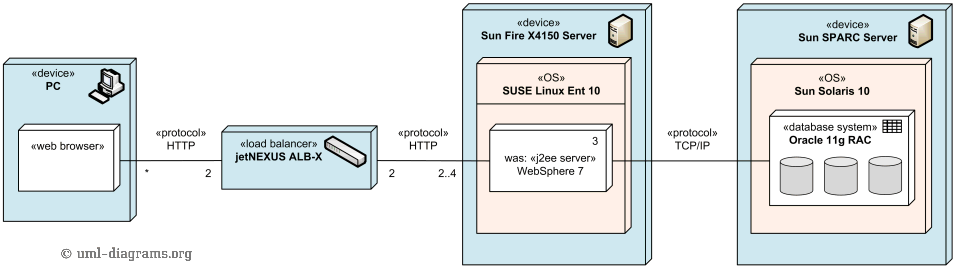
\includegraphics[width=\textwidth]{img/deployment-diagram-2.png}
    \caption{Deployment Diagram.}
\end{figure}

\noindent
To view the sequence diagram in high resolution, scan (or click) the QR code below.
\begin{center}
    \qrcode{https://github.com/PoliMI-HPC-E-notes-projects-AndreVale69/HPC-E-PoliMI-university-notes/tree/main/software-engineering-for-hpc/notes/img/deployment-diagram.png}
    \hspace{2em}
    \qrcode{https://github.com/PoliMI-HPC-E-notes-projects-AndreVale69/HPC-E-PoliMI-university-notes/tree/main/software-engineering-for-hpc/notes/img/deployment-diagram-2.png}
\end{center}
A complete guide can be found on the following page: \href{https://www.visual-paradigm.com/guide/uml-unified-modeling-language/what-is-deployment-diagram/}{What is Deployment Diagram?
}